\begin{sectionbox}
Is a method that makes use of geometrical aspects in order to solve \imp{\nth{1}-order PDEs} with two variables of the type:
\setspacing{0pt}
    \begin{alignat}{5}
        &\text{\rd{Linear}: }&          &\mc{a}(x,y)\vec{u}_x&+           &\mc{b}(x,y)\vec{u}_y           &=&\mc{c}(x,y)
            \label{eq:moc1}     \nalign
        &\text{\rd{Semilin}.: }&    &\mc{a}(x,y)\vec{u}_x&+           &\mc{b}(x,y)\vec{u}_y           &=&\mc{c}(x,y,\vec{u})
            \label{eq:moc2}\nalign
        &\text{\rd{Quasilin}.: }&       &\mc{a}(x,y,\vec{u})\vec{u}_x&+&\mc{b}(x,y,\vec{u})\vec{u}_y&=&\mc{c}(x,y,\vec{u})
            \label{eq:moc3}
    \end{alignat}
\end{sectionbox}
\subsection{Linear Equations}
\begin{sectionbox}
The solution $\vecu(x,y)$ of \cref{eq:moc1} can be sought of as an surface $z=\vecu(x,y)$ in $\R^3$ or in implicit form
    $\phi(x,y,z):=\vecu(x,y)-z$.
    \begin{figure}[H]
        \centering{
            \def\svgwidth{100pt}
            \resizebox{0.6\linewidth}{!}{\input{figures/integral_surface.pdf_tex}}
        }
    \end{figure}
\imp{Let}:$\tulm[2]{\vec{n}(x,y)}:=\grad\phi=\vect{\phi_x \\ \phi_y \\ \phi_z}=\vect{\vecu_x \\ \vecu_y \\ -1}$\hfil\imp{and}\\
    \imp{Let}: $\mc{\vec{V}}:=\vect{\mc{a}(x,y) \\ \mc{b}(x,y) \\ \mc{c}(x,y)}$ be a vector field $\R^3\mapsto\R^3$.\\
\imp{Idea}: we can rewrite \cref{eq:moc1} as:\\
$\left\langle\vect{\mc{a} & \mc{b} & \mc{c}}^\top,\nabla\phi(x,y,z)\right\rangle=
    \left\langle\vect{\mc{a}(x,y) \\ \mc{b}(x,y) \\ \mc{c}(x,y)},\tulm[2]{\vect{\vecu_x \\ \vecu_y \\ -1}}\right\rangle=0$
\begin{proofbox}
    \begin{proof}
        $\vec{n}\cdot\vec{v}=0\Leftrightarrow\mc{a}\vecu_x+\mc{b}\vecu_y-\mc{c}=0\Leftrightarrow\cref{eq:moc1}$
    \end{proof}
\end{proofbox}
\imp{Geometric Interpretation}:
$\mc{\vec{v}}$ is orthogonal to the normal $\tulm[2]{\vec{n}}$ for all points $(x,y,\vecu(x,y))$.\\
\imp{Hence} every vector $\mc{\vec{v}}=\vect{\mc{a} & \mc{b} & \mc{c}}^\top$ lies in the tagent plane containing $\phi$.
\end{sectionbox}
\begin{defnbox}
    \begin{defn}[Integral Surface]\label{Integral Surface}
        An function $\phi$ is a an integral surface of a vector field $\mc{\vec{V}}$\\
        $\iff\phi$ is a surface that has in every point a tangent plane containing a vecetor \mc{\vec{v}}=\vect{\mc{a}&\mc{b}&\mc{c}} of $\mc{\vec{V}}$.
    \end{defn}
\end{defnbox}
\begin{sectionbox}
\begin{wrapfigure}[5]{r}{0.4\linewidth}
    \centering{
        \inkscape[80pt]{figures/integral_curve.pdf_tex}
    }
\end{wrapfigure}
\imp{Consequently} in order to find a surface $\phi$ (and thus also a solution $\vecu$), we need to search for $\phi$ s.t.
the vector $\mc{\vec{v}}$ lies in the tangent plane for every possible point of $\phi$.\\
\imp{Idea}: we first simplify the task and start by constructing/finding integral curves $\mc[5]{\gamma}$ and
then we constructe the integral surface $\phi$ out of this curves.
\end{sectionbox}
\begin{defnbox}
    \begin{defn}[Integral Curve]\label{Integral Curve}
        Is a curve $\mc[5]{\gamma}$ parameterized by $r$ of a vector field $\mc{\vec{V}}$ s.t. at each point of:\\
        \ctr{$\mc[5]{\gamma}(r):=x(r)\vec{e}_x+y(r)\vec{e}_y+z(r)\vec{e}_z=\vect{x(r)\\y(r)\\z(r)}$}
        the vector:\\
        \ctr{$\mc{\vec{v}}=\vect{\mc{a}(x(r),y(r)) & \mc{b}(x(r),y(r)) & \mc{c}(x(r),y(r))}$}\\
        is tangent to the curve.
    \end{defn}
\end{defnbox}
\begin{sectionbox}
\imp{Thus} such an integral curve $\gammac$ must satisfy:\\
\ctr{
    $\frac{\diff \gammac(r)}{\diff r}=\mc{\vec{V}}(\gammac(r))=
    \vect{\tulm[5]{\mc{a}\big(x(r),y(r)\big)} \\ \tulm[5dashed]{\mc{b}\big(x(r),y(r)\big)} \\ \tulm[5dotted]{\mc{c}\big(x(r),y(r)\big)}}=
    \vect{\mc{a}(\gammac(r)) \\ \mc{b}(\gammac(r)) \\ \mc{c}(\gammac(r))}$
    }\\
This leads to a set of ordinary differential equations known as characteristic equations:
\end{sectionbox}
\begin{defnbox}
    \begin{defn}[Characteristic Equations]\label{Characteristic Equations}
        \nospacing
        \begin{align}
            \frac{\partial x(r)}{\partial r}=\dot{x}=\tulm[5]{\mc{a}(\gammac(r))}=\mc{a}(r) \nalign
            \frac{\partial y(r)}{\partial r}=\dot{y}=\tulm[5dashed]{\mc{b}(\gammac(r))}=\mc{b}(r) \nalign
            \frac{\partial z(r)}{\partial r}=\dot{z}=\tulm[5dotted]{\mc{c}(\gammac(r))}=\mc{c}(r)
        \end{align}
    \end{defn}
\end{defnbox}
\begin{notebox}[Example \normalfont{$u_x+\mc{b}u_y=0$}]
    \imp{ODEs}:\hfil
        $\frac{\diff x}{\diff r}=1$\hfil
        $\frac{\diff y}{\diff r}=\mc{b}$\hfil
        $\frac{\diff u}{\diff r}=0$\hfil
        $\left[\Rightarrow\vect{1 & \mc{b}}\cdot\nabla u\stackrel{!}{=}0\right]$\\
    \imp{Thus}:\hfil
        $x(r)=\tulm[4]{r}+c_1$\hfil
        $y(r)=\tulm[4]{r}\mc{b}+c_2$\hfil
        $u(r)=f(\tulm[6]{c_3})$\\
    $\Rightarrow\tulm[4]{r}=x-c_1$\hfil $\Rightarrow y=(\tulm[4]{x-c_1})\mc{b}+c_2=x\mc{b}+\tulm[6]{c_3}$\\
    \ctr{$\Rightarrow u(x,y)=f(\tulm[6]{y-x\mc{b}})$}
\end{notebox}
\begin{notebox}[Note]
    Thus $u$ is constant along curves in the direction $\vect{1 & \mc{b}}$, that is $u$ is constant along the lines
    $y=x\mc{b}+c_3$ for any function $f(c_3)$:
 \end{notebox}
\begin{sectionbox}
    \imp{Problem}: in order to get a unique solution we need to specify initial conditions.\\
    \imp{Idea}: If a characteristc has an arbitrary point in common with the integral surface $\phi$ then the whole characteristic
                $\gammac$ will lie in the integral surface.
    \begin{proofbox}
        \begin{proof}
        \nospacing
            \imp{Let}: $\phi(\gammac(r))=u(x(r),y(r))-z(r)$
            \begin{align*}
                \Rightarrow\frac{\diff \phi}{\diff r}
                &=u_x\tulm[5]{\frac{\diff x}{\diff r}}
                    +u_y\tulm[5dashed]{\frac{\diff y}{\diff r}}
                    -1\tulm[5dotted]{\frac{\diff z}{\diff r}}=           \nalign
                &=\vect{u_x \\ u_y \\ -1}\vect{\mc{a}\big(x(r),y(r)\big) \\ \mc{b}\big(x(r),y(r)\big) \\ \mc{c}\big(x(r),y(r)\big)}
                    =\vect{u_x \\ u_y \\ -1}\dot{\gammac}(r)=0
            \end{align*}
            \imp{Thus}: $\phi(\gammac(r_0))=0\iff\phi(\gammac(r))=0,\ \forall r$
        \end{proof}
    \end{proofbox}
\end{sectionbox}
    \begin{defnbox}
        \begin{defn}[Characteristic \tc{Black}{(}Curve\tc{Black}{)}] $\gammac_s(r)=\gammac(r;s)$ is a integral curve of the vector field $\mc{\vec{V}}$ that is uniequely determined by a parameter $s$.
        \end{defn}
    \end{defnbox}
\begin{sectionbox}
    \begin{wrapfigure}[17]{r}{0.4\linewidth}
        \centering{
            \inkscape[80pt]{figures/integral_surface_initial_condition.pdf_tex}
        }
    \end{wrapfigure}
    \imp{Consequence}: For every characteristic $s$ we need to specify one inital point on the integral surface in order to have all the characteristics lie within the integralsurface.\\
    \imp{Idea}: we define another curve $\tc{Brown}{\Gamma}(s)$ on the integralsurface that transvers all the characteristic curves
     $\gammac_s(r)$ \rd{transversal}
     (=angle beetween $\tc{Brown}{\Gamma}(s)$ and $\gammac_s(r)$ is never zero $\Leftrightarrow \tc{Brown}{\Gamma}(s)\nparallel\gammac_s(r)$).
\end{sectionbox}
\begin{defnbox}
    \begin{defn}[Inital Condition]
        $s\mapsto\tc{Brown}{\Gamma}(s),\ \tc{Brown}{\Gamma}:\R\mapsto\R^3$\\
        $\gammac_s(r)=\vect{\tulm[dotted]{\gammac[x]_s}(r) \\ \tulm[2dotted]{\gammac[y]_s}(r) \\ \tulm[3dotted]{\gammac[z]_s}(r)}$,\quad
        $\tc{Brown}{\Gamma}(s)=\vect{\tulm[1]{\tc{Brown}{x}_0(s)} \\\tulm[2]{\tc{Brown}{y}_0(s)} \\\tulm[3]{\tc{Brown}{z}_0(s)}}$\hfill
        $\gamma_s(0)\stackrel{!}{=}\tc{Brown}{\Gamma}(s)$\\
        $\Rightarrow \tulm[dotted]{x_s}(0)=\tulm[1]{x_0(s)}$\hfil
        $\tulm[2dotted]{y_s}(0)=\tulm[2]{y_0(s)}$\hfil
        $\tulm[3dotted]{z_s}(0)=\tulm[3]{z_0(s)}$
    \end{defn}
\end{defnbox}
\begin{defnbox}
    \begin{defn}[Projected Characteristic Curves]
        Are the curves $\gammac[y]_s(x)$ in the $yx$-plane (resp. $\gammac[x]_s(t)$ in the $xt-plane$) along which u is constant
        (for ODEs as $\frac{\partial u}{\partial r}=$constant) or satisfies certain conditions.\\
        The initial data/information is simply propagated along those characteristic curves.
    \end{defn}
\end{defnbox}
\begin{notebox}[Example 2: \textnormal{$5u_t+2u_x=0$\hfil $\dot{t}=5,\ \dot{x}=2t,\ \dot{z}=0$}]
                \imp{Initial Conditions}:\hfil $u(x, 0)=\tulm[3]{\psi}(\tulm{x})$\\
                $\Rightarrow$\hfil $\vect{5 & 2}\cdot\nabla u=0$\\
                \imp{Parameterisation}:\\
                $\Rightarrow u(\tulm[dotted]{x_s(r)},\tulm[2dotted]{t_s(r)})=\gammac[z]_s(0)=\tc{Brown}{z}_0(s)=u(\tulm[1]{s},\tulm[2]{0})=\tulm[3]{\psi}(\tulm{s})$\\
                $\Rightarrow \gammac[x]_s(0)=\tc{Brown}{x}_0(s)=\tulm{s},\
                             \gammac[t]_s(0)=\tc{Brown}{t}_0(s)=\tulm[2]{0}$
\end{notebox}
\begin{notebox}[Solution 2]
                \nospacing
                \begin{alignat*}{3}
                    &\gammac[t]_s=5r+c_1(s)                      &  & \gammac[t]_s(0)=c_1(s)=0       & & \gammac[t]_s=5\tulm[4]{r}\\
                    &\gammac[x]_s=2r+c_2(s)     \Rightarrow\quad &  & \gammac[x]_s(0)=c_2(s)=s           &\Rightarrow\ \ & \gammac[x]_s=2\tulm[4]{r}+\tulm[5]{s}      \\
                    &\gammac[z]_s=c_3(s)                     &  & \gammac[z]_s(0)=c_3(s)=\phi(s) &                    & \gammac[z]_s=\phi(\tulm[5]{s})
                \end{alignat*}
                $\Rightarrow$\hfil$ \gammac_s(r)=\vect{5r & 2r+s & \psi(\tulm[5]{s})}$\\
                \imp{Now} we need the inverse transformation $r(x,t),\ s(x,t)$
                $\Rightarrow \gammac[t]_s=5r \Leftrightarrow \tulm[4]{r}=\frac{t}{5}$\qquad
                    $\Rightarrow  \gammac[x]_s=2\tulm[4]{\frac{t}{5}}+\tulm[5]{s} \Leftrightarrow \tulm[5]{s}=x-\frac{2}{5}t$\\
                \imp{Thus}: \ctr{$u(x,t)=\psi(\tulm[5]{x-\frac{2}{5}t})$}
\end{notebox}
\begin{notebox}[Note]
    $x_s(t)=\frac{2}{5}t+s$ are the porjected characteristic curves \cref{fig:projChar1p1} which are constant along $\frac{\diff x}{\diff t}=\frac{2}{5}t$.
                \begin{figure}[H]
                    \centering
                    \begin{subfigure}{.4\columnwidth}
                      \centering
                      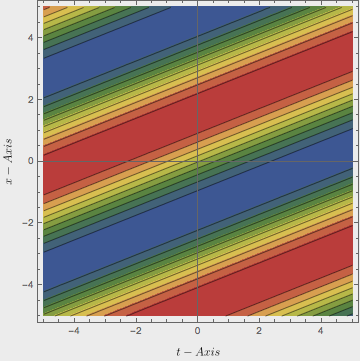
\includegraphics[width=\linewidth]{figures/projChar1p1.png}
                      \caption{proj. Char.}
                      \label{fig:projChar1p1}
                    \end{subfigure}%
                    \begin{subfigure}{.6\columnwidth}
                      \centering\tabularnewline
                      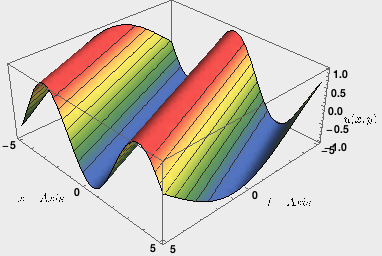
\includegraphics[width=\linewidth]{figures/projChar1p2.png}
                      \caption{Solution Surface}
                      \label{fig:projChar1p2}
                    \end{subfigure}
                    \caption{$\psi(s)=\sin(s)$}
                \end{figure}
\end{notebox}

\begin{notebox}[Example 3: \textnormal{$5u_t+2tu_x=0$\hfil $\dot{t}=5,\ \dot{x}=2t,\ \dot{z}=0$}]
                \imp{Initial Conditions}:\hfil $u(x, 0)=\tulm[3]{\sin}(\tulm{x})$\\
                $\Rightarrow$\hfil $\vect{5 & 2t}\cdot\nabla u=0$\\
                \imp{Parameterisation}:\\
                $\Rightarrow u(\tulm[dotted]{x_s(r)},\tulm[2dotted]{t_s(r)})=\gammac[z]_s(0)=\tc{Brown}{z}_0(s)=u(\tulm[1]{s},\tulm[2]{0})=\tulm[3]{\sin}(\tulm{s})$\\
                $\Rightarrow \gammac[x]_s(0)=\tc{Brown}{x}_0(s)=\tulm{s},\
                             \gammac[t]_s(0)=\tc{Brown}{t}_0(s)=\tulm[2]{0}$
\end{notebox}
\begin{notebox}[Solution 3]
                \nospacing
                \begin{alignat*}{3}
                    &\gammac[t]_s=5r+c_1(s)                  &  &\xrightarrow{\gammac[t]_s(0)=0} &   & \tulm[6]{\gammac[t]}_s=5\tulm[4]{r}\\
&\dot{\gammac[x]}_s=2\tulm[6]{t}\Rightarrow\gammac[x]_s=5r^2+c_2(s)&    &\xrightarrow{\gammac[x]_s(0)=s}  &  & \gammac[x]_s=5\tulm[4]{r}^2+\tulm[5]{s}      \\
                    &\gammac[z]_s=c(3)_s                 &\     &\xrightarrow{\gammac[z]_s(0)=\sin(s)}&\ & \gammac[z]_s=\sin(\tulm[5]{s})
                \end{alignat*}
                $\Rightarrow$\hfil$ \gammac_s(r)=\vect{5r & 2r^2+s & \psi(\tulm[5]{s})}$\\
                \imp{Now} we need the inverse transformation $r(x,t),\ s(x,t)$
                $\Rightarrow \gammac[t]_s=5r \Leftrightarrow \tulm[4]{r}=\frac{t}{5}$\qquad
                    $\Rightarrow  \gammac[x]_s=5\tulm[4]{\left(\frac{t}{5}\right)^2}+\tulm[5]{s} \Leftrightarrow
                    \tulm[5]{s}=x-\frac{t^2}{5}$\\
                \imp{Thus}: \ctr{$u(x,t)=\sin(\tulm[5]{x-\frac{t^2}{5}})$}
\end{notebox}
\begin{notebox}[Note]
    $x_s(t)=\frac{1}{5}t^2+s$ are the porjected characteristic curves \cref{fig:projChar2p1} which are constant along $\frac{\diff x}{\diff t}=\frac{2}{5}t$.
                \begin{figure}[H]
                    \centering
                    \begin{subfigure}{.4\columnwidth}
                      \centering
                      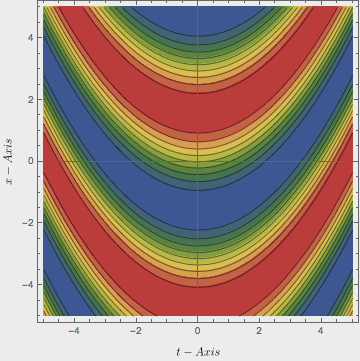
\includegraphics[width=\linewidth]{figures/projChar2p1.png}
                      \caption{proj. Char.}
                      \label{fig:projChar2p1}
                    \end{subfigure}%
                    \begin{subfigure}{.6\columnwidth}
                      \centering\tabularnewline
                      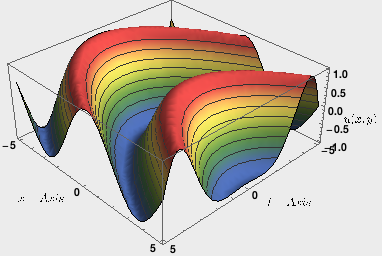
\includegraphics[width=\linewidth]{figures/projChar2p2.png}
                      \caption{Solution Surface}
                      \label{fig:projChar2p2}
                    \end{subfigure}
                \end{figure}
\end{notebox}
\begin{stylebox}
\nospacing
\sectionHeader{Hint}: If the PDE is linear, then the two first characteristics do not depend on u and can be solved directly,
u will then be constant along those characteristics:
\begin{alignat*}{5}
    &\mc{a}(x,y)\vec{u}_x&+&\mc{b}(x,y)\vec{u}_y&=&\mc{c}(x,y) \nalign
    &\frac{\diff x}{\diff r}=\mc{a}&
    &\frac{\diff y}{\diff r}=\mc{b}&
    &\frac{\diff u}{\diff r}=\mc{c}&
    \quad\text{\imp{implies}}&
\quad\frac{\diff y}{\diff x}=\frac{\mc{b}(x,y)}{\mc{a}(x,y)}
\end{alignat*}
\end{stylebox}
\begin{stylebox}
\sectionHeader{Hint}: If we divide the PDE by $\mc{a}$ we have to solve a PDE less, beacause the first ODE will allways be:\\
$\dot{x}=\mc{1}\Rightarrow$\hfil$ x=r
\Rightarrow$\hfil$ \gammac[x]_s(r)=\tc{Brown}{x}_0(s)$
\end{stylebox}


\subsection{Quasilinear Equations}
\begin{sectionbox}[\subsubsection*{Solving Quasilinear Equations}]
\nospacing
    \begin{alignat*}{5}
        &\mc{a}(x,y,u)\vec{u}_x&+&\mc{b}(x,y,u)\vec{u}_y&=&\mc{c}(x,y,u) \\
        &u_{\mid\tc{Brown}{\Gamma}}(r,s)=\phi(s) \\
        &\frac{\diff x}{\diff r}=\mc{a}(x,y,u)&
        &\frac{\diff y}{\diff r}=\mc{b}(x,y,u)&
        &\frac{\diff u}{\diff r}=\mc{c}(x,y,u)          \nalign
        & \gammac[x]_s(0)=\tc{Brown}{x}_0(s)&
        & \gammac[y]_s(0)=\tc{Brown}{y}_0(s)&
        & \gammac[z]_s(0)=\phi(s)
    \end{alignat*}
\end{sectionbox}
\begin{sectionbox}[Results]
Now the projected characteristic curves may depend on u as well as on x,y.
\imp{Thus} the first two characteristics are no longer decoupled form the third one.
    \begin{numberlist}
        \item We may get projected characteristic curves crossing themselfs.
        \item u is no longer constant along the projected characteristic curves, rather the PDE reduces to an ODE satisfying
        certain conditions along this curves.
    \end{numberlist}
\end{sectionbox}


\subsubsection{Transversality Condition}
\begin{defnbox}
    \begin{defn}[Cauchy Problem]\leavevmode \\
        \ctr{$\mc{a}(x,y)u_x+\mc{b}(x,y)u_y=\mc{x}$\hfil in $\Omega\bdla{=}{\normalfont{Cauchy Problem}}\R^n$}\\
        \ctr{$u_{\mid\tc{Brown}{\Gamma}}=\psi$}
    \end{defn}
\end{defnbox}
\begin{sectionbox}[Question]
    Is the \rd{Cauchy Problem} well posed for all
    $\tc{Brown}{\Gamma}$ in $\R^2$?\\
    \imp{No}: if the initial curve transvers the projected characteristics:
        \begin{numberlist}
            \item \imp{Not transversal}
            \item \imp{More than once}
        \end{numberlist}
        Then the values of u will not be unique.
\end{sectionbox}
\begin{sectionbox}[Problem]
\nospacing
    We parameterized the characteristics s.t.:\\
    \ctr{$\gammac[z](r;s)=u(\gammac[x](r;s),\gammac[y](r;s))$\hfil$\Leftrightarrow$\hfil$ \Psi(r,s)\mapsto(x(r,s),y(r,s))$}\\
    but if the \rd{transversality condition} (\cref{Transversality Condition}) is not satisfied , then their will be no mapping\\
    \ctr{$\Psi^{-1}:(\gammac[x],\gammac[y])\mapsto(r(\gammac[x],\gammac[y]);s(\gammac[x],\gammac[y]))$}\\
    and thus we will not be able to find the solution.
        \begin{figure}[H]
            \centering
            \begin{subfigure}{.5\columnwidth}
                \centering{
                    \def\svgwidth{100pt}
                    \resizebox{\linewidth}{!}{\input{figures/transversality1.pdf_tex}}
                }
                \caption{\imp{Problem 1}: \rd{Transversality}\\ for characteristic at\\ $(t,x)=(0,0)$}
            \end{subfigure}%
            \begin{subfigure}{.5\columnwidth}
                \centering{
                    \def\svgwidth{100pt}
                    \resizebox{\linewidth}{!}{\input{figures/transversality2.pdf_tex}}
                }
                \caption{\imp{Problem 2}: \rd{Uniquness} have to chose either upper or lower ray in order to get a unique solution.}
            \end{subfigure}
        \end{figure}
\end{sectionbox}
\begin{lemmabox}
\nospacing
    \begin{lemma}[Transversality Conditions for Semi-and Quasilinear-equations]\label{Transversality Condition2}\leavevmode \\
        \begin{align}
            \det(J_\Psi)&=\det\bmat{
                \frac{\partial \gammac[x]_s(r)}{\partial r} & \frac{\partial \gammac[x]_s(r)}{\partial s} \\
                \frac{\partial \gammac[y]_s(r)}{\partial r} & \frac{\partial \gammac[y]_s(r)}{\partial s}}
                =\det\bmat{
                \mc{a} &  \Big(\gammac[x]_s(r)\Big)_s\\
                \mc{b} &  \Big(\gammac[y]_s(r)\Big)_s } \nonumber   \nalign
                &=\mc{a}\cdot\Big(\gammac[x]_s(r)\Big)_s-\mc{b}\cdot\Big(\gammac[y]_s(r)\Big)_s\ne0
        \end{align}
    \end{lemma}
\end{lemmabox}
\begin{sectionbox}[\subsubsection{Case Studie: Burgers Equation}]
\nospacing
    \begin{alignat}{3}
        &u_t+u u_x&=&0 \nonumber\nalign
        &u(x,0)&=&\Phi(x)\label{eq:Burgers Equation}
    \end{alignat}
    \begin{alignat*}{5}
    &\imp{\text{ODEs}}         &\qquad          &\frac{\diff t}{\diff r}=1 &       &\frac{\diff x}{\diff r}=\tulm{u}&          &\frac{\diff u}{\diff r}=0   \nalign
    &\imp{\text{I.C.}}         &\qquad          &\gammac[t](0;s)=0  &\qquad &\gammac[x](0;s)=s           &\qquad   &\gammac[u](0;s)=\Phi(s)
    \end{alignat*}
    \imp{Solution}          \hfil $\gammac[t]_s(r)=r+c_1(s)$\hfil    $\gammac[u]_s(r)=\tulm{c_3(s)}$\\
    $\Rightarrow \frac{\diff x}{\diff r}=\tulm{c_3(s)}$\hfil $\Rightarrow\gammac[x]_s(r)=\tulm{c_3(s)}r+c_2(s)$\\
    \imp{I.C.} \hfil $\gammac[t]_s(r)=r$\hfil $\gammac[u]_s(r)=\tulm{\Phi(\tulm[2]{s})}$\hfil $\gammac[x]_s(r)=\tulm{\Phi(s)}r+\tulm[2]{s}$\\
    \imp{Invers} \hfil $r=t$\hfil $\tulm[2]{s}=x-\phi(s)r=x-\phi(s)t=x-ut$\\
    \imp{Thus}\hfil $u(x,t)=\phi(\tulm[2]{x-ut})$\\
    \imp{With} \rd{proj. characteristics}:\hfil $x_{\mc[3]{s}}=\bdra{\phi(\mc[3]{s})}{\normalfont{slope/speed}}t+\mc[3]{s}$
\end{sectionbox}
\begin{sectionbox}[Geometric Interpretation]
    $\phi(\mc[3]{s})$ determines the speed of a characteristic emanating from a given $\mc[3]{s}$:\hfil
    $\begin{cases}
        x=kt+d      \\
        x_{\mc[3]{s}}=\phi(\mc[3]{s})t+\mc[3]{s}  \\
    \end{cases}$
\end{sectionbox}
\begin{notebox}[Consequences]
    \begin{wrapfigure}{l}{0.5\linewidth}
        \centering{
            \inkscape[90pt]{figures/crit_speed.pdf_tex}
        }
    \end{wrapfigure}
\imp{Suppose} there exists $\mc[3]{s}_1<\mc[3]{s}_2$ s.t. $\phi(\mc[3]{s}_1)>\phi(\mc[3]{s}_2)$.\\
\imp{Then} the proj. char. curves $x_{\mc[3]{1}}, x_{\mc[3]{2}}$ will intersect at some point $(x_0,t_0)$.\\
$\Rightarrow$ \imp{Problem}: because at $(x_0,t_0)$ we will no longer have a unique solution. This can also be seen by the transversality condition (\cref{Transversality Condition2}):\\
\end{notebox}
\begin{emphbox}
\nospacing
$\Psi(t(r,s),x(r,s))=\Psi(r,\phi(s)r+s)$\\
    \begin{align*}
            \det(J_\Psi)&=\det\bmat{
                \mc{a} &  \Big(\gammac[t]_s(r)\Big)_s\\
                \mc{b} &  \Big(\gammac[x]_s(r)\Big)_s }
                =\bmat{
                1       &  0\\
                \phi(s) &  \phi'(s)r+1 }    \nalign
                &=\phi'(s)r+1\stackrel{!}{\ne}0
        \end{align*}
        \[\Rightarrow \det(J_\Psi)=0 \iff r=-\frac{1}{\phi'(s)}\qquad t_{\rd{\text{crit}}}=-\frac{1}{\phi'(s)}\]
\end{emphbox}
\begin{notebox}[What happens at $t_{\rd{crit}}$?]
\nospacing
    From $u=\phi(x-ut)$ we find $u_x=\phi_x\cdot(1-t u_x)$\\
    \[\Rightarrow u_x=\frac{\phi'}{1+t\phi'}\qquad\Rightarrow u_x(t_{\rd{crit}})=\frac{\phi'}{1+t_{\rd{crit}}\phi'}=\infty\]
    \imp{Thus} the derivitative of the solution blows up at a the critical time and the \rd{classical solution} is no longer defined for $t\ge t_{\rd{crit}}$.
\end{notebox}
\begin{defnbox}
    \begin{defn}[Classical/Strong Solution]\leavevmode \\
        Let $\vecu$ satisfy the PDE $\FT\big(\vecu,D\vecu,\ldots,D^k\vecu,\mc[2]{f}\big)=0$ of order $k$.\\
        $\vecu$ is called a strong solution $\iff \vecu$ is at least $k$-times differentiable $u\in C^k$.
    \end{defn}
\end{defnbox}
\begin{defnbox}
    \begin{defn}[Shockwave]\leavevmode \\
        Is the formation of a singularity at a critical time $t_{\rd{crit}}$.
    \end{defn}
\end{defnbox}
\begin{notebox}[Minimum requirement for a shockwave]
    A neccessary condition is that $\phi(s)<(0)$ at least at some point s.t. a faster characteristic will start from a point
    behind a slower one. If $\phi(s)$ is never decreasing there will never be a singularity
    $\frac{\diff y}{\diff y}=\frac{\phi(r_2)-\phi(r_1)}{r_2-r_1}<0$
    \todo[inline]{Check if this is correct or just humbug}
\end{notebox}
\begin{notebox}[Physical Interpretation]
 At the singularity (\rd{shockwave}) $t=t_{\rd{crit}}$ the faster characteristic (taller part of a wave) will overtake the slower one
 (shorter part of wave), causing the wave to break.
    \begin{figure}[H]
        \centering{
            \def\svgwidth{150pt}
            \resizebox{0.8\linewidth}{!}{\input{figures/waves.pdf_tex}}
        }
    \end{figure}
    \imp{Thus} their exists a phisical meaning after $t_{\rd{crit}}$ where the \rd{classical solution} does not exist anymore.\\
    \imp{Question}: If there exists no \rd{strong solution} is there a way to find another solution?
\end{notebox}
\begin{emphbox}[Recap Method of Characteristics]\leavevmode\\
    $x:=x(r;s)$\hfil$y:=y(r;s)$\hfil$z:=u(r;s)$\\
    \imp{Parameter.}:\hfil$\gammac(r;s):=x(r;s)\vec{e}_x+y(r;s)\vec{e}_y+z(r;s)\vec{e}_z$\\
    \ctr{$\frac{\partial \gammac}{\partial r}(r;s)=(\mc{a},\mc{b},\mc{c})$}\\
    \imp{E.g.} \ctr{$\mc{v}:=\mc{v}(x(r;s),y(r;s),z(r;s))$}
    \ctr{$\frac{\partial x}{\partial r}(r;s)=\dot{x}=\mc{a}(\gammac_s(r))$}\\
    \ctr{$\frac{\partial y}{\partial r}(r;s)=\dot{y}=\mc{b}(\gammac_s(r))$}\\
    \ctr{$\frac{\partial z}{\partial r}(r;s)=\dot{z}=\mc{c}(\gammac_s(r))$}
\end{emphbox}
\begin{emphbox}
    \imp{Compact}:\hfil $\dot{x}=\mc{a}(x,y,u)$\hfil $\dot{y}=\mc{b}(x,y,u)$\hfil $\dot{u}=\mc{c}(x,y,u)$\\
    \imp{I.C.}:\hfil $x(0;s)=x_0(s)$\hfil $y_0(0;s)=y_0(s)$\hfil $u(0;s)=u_0(s)$
\end{emphbox}

%%% Local Variables:
%%% mode: latex
%%% TeX-command-extra-options: "-shell-escape"
%%% TeX-master: "../../formulary"
%%% End:
